\documentclass[11pt]{beamer}
\usepackage{ctex}
\usepackage[utf8]{inputenc}
\usepackage[T1]{fontenc}
\usepackage{lmodern}
\usepackage{listings}
\usepackage{frame}
\usetheme{CambridgeUS}


\begin{document}
%	\author{}
	\title{\LaTeX 入门}
	\subtitle{第1章 熟悉Latex}
	%\logo{}
	%\institute{}
	\date{2022年8月1日}
	%\subject{}
	%\setbeamercovered{transparent}
	%\setbeamertemplate{navigation symbols}{}
	\begin{frame}[plain]
		\maketitle
	\end{frame}
	
	
\begin{frame}{熟悉\LaTeX}
	\LaTeX 是一种文档排版系统。\\
	\LaTeX 是现在最流行的科技写作——尤其是数学写作的工具之一。
\end{frame}

\part{让\LaTeX 跑起来}

\begin{frame}{让\LaTeX 跑起来}
	Tex Live \\ Tex Studio \\ (VSCode) \\ Overleaf
\end{frame}

\section{Happy \TeX ing}

\begin{frame}[fragile]{让\LaTeX 跑起来}{Happy \TeX ing}
	\begin{verbatim}
		\documentclass{article}
	
		\begin{document}
		This is my first document.
			
		Happy \TeX ing!
		\end{document}
	\end{verbatim}
\end{frame}

\section{特可爱排版}

\begin{frame}[fragile]{让\LaTeX 跑起来}{特可爱排版}
	\begin{verbatim}
		\documentclass[UTF8]{ctexart}
		\begin{document}
		\section{文字}
		特可爱排版。
		\section{数字}
		\[
			a^2 + b^2 = c^2
		\]
		\end{document}
	\end{verbatim}
\end{frame}

\section{命令行}

\begin{frame}[fragile]{让\LaTeX 跑起来}{命令行}
	\begin{verbatim}
		latex demo.tex
		pdflatex demo.tex
		xelatex demo.tex
		lualatex demo.tex
	\end{verbatim}
\end{frame}

\part{从一个例子说起}

\section{从提纲开始}

\begin{frame}[fragile]{从一个例子说起}{从提纲开始}
	\begin{columns}
	\begin{column}{.5\linewidth}\begin{verbatim}
		%-*- coding: UTF-8 -*-
		% gougu.tex
		% 勾股定理
		\documentclass[UTF8]{ctexart}
		
		\title{杂谈勾股定理}
		\author{张三}
		\date{\today}
	\end{verbatim}\end{column}

	\begin{column}{.5\linewidth}\begin{verbatim}
		\bibliographystyle{plain}
	
		\begin{document}
			\maketitle
			\tableofcontents
			\section{勾股定理在古代}
			\section{勾股定理的近代形式}
			%	\bibliography{math}
		\end{document}
	\end{verbatim}\end{column}

	\end{columns}
\end{frame}

\section{填写正文}

\begin{frame}[fragile]{从一个例子说起}{填写正文}
	\begin{verbatim}
		西方称勾股定理为毕达哥拉斯定理,将勾股定理的发现归功于公元前 6 世纪的毕达哥拉斯学派。该学派得到了一个法则,可以求出可排成直角三角形三边的三元数组。毕达哥拉斯学派没有书面著作,该定理的严格表述和证明则见于欧几里德《几何原本》的命题 47:“直角三角形斜边上的正方形等于两直角边上的两个正方形之和。”证明是用面积做的。
		
		我国《周髀算经》载商高(约公元前 12 世纪)答周公问……
	\end{verbatim}
\end{frame}

\section{命令与环境}

\begin{frame}[fragile]{从一个例子说起}{命令与环境}
	\begin{verbatim}
		……见于欧几里德\footnote{欧几里德,约公元前 330--275 年。}《几何原本》的……
		
		……的整数称为\emph{勾股数}。
		
		……答周公问:
		\begin{quote}
		勾广三,股修四,径隅五。
		\end{quote}
		又载陈子(约公元前 7--6 世纪)答荣方问:
		\begin{quote}
		若求邪至日者,以日下为勾,日高为股,勾股各自乘,并而开方除之,得邪至日。
		\end{quote}
		都较古希腊更早。……
	\end{verbatim}
\end{frame}

\begin{frame}[fragile]{从一个例子说起}{命令与环境}
	\begin{verbatim}
		\begin{quote}
		\zihao{-5}\kaishu 引用的内容。

		\end{quote}
	\end{verbatim}
\end{frame}

\begin{frame}[fragile]{从一个例子说起}{命令与环境}
	\begin{verbatim}
		\begin{abstract}
		这是一篇关于勾股定理的小短文。
		\end{abstract}
	\end{verbatim}
\end{frame}

\begin{frame}[fragile]{从一个例子说起}{命令与环境}
	\begin{verbatim}
		\newtheorem{thm}{定理}% 导言区
		
		\begin{thm}[勾股定理]
		直角三角形斜边的平方等于两腰的平方和。
		
		可以用符号语言表述为……
		\end{thm}
	\end{verbatim}
\end{frame}

\section{遭遇数学公式}

\begin{frame}[fragile]{从一个例子说起}{遭遇数学公式}
	\begin{verbatim}
		\begin{equation}
			a(b+c) = ab + ac
		\end{equation}
	
		$\angle ACB = \pi / 2$
		
		\begin{equation}
		AB^2 = BC^2 + AC^2
		\end{equation}
	\end{verbatim}
\end{frame}

\section{使用图表}

\begin{frame}[fragile]{从一个例子说起}{使用图表}
	\begin{verbatim}
		\documentclass{ctexart}
		\usepackage{graphicx}
		% ……导言区其他内容
		
		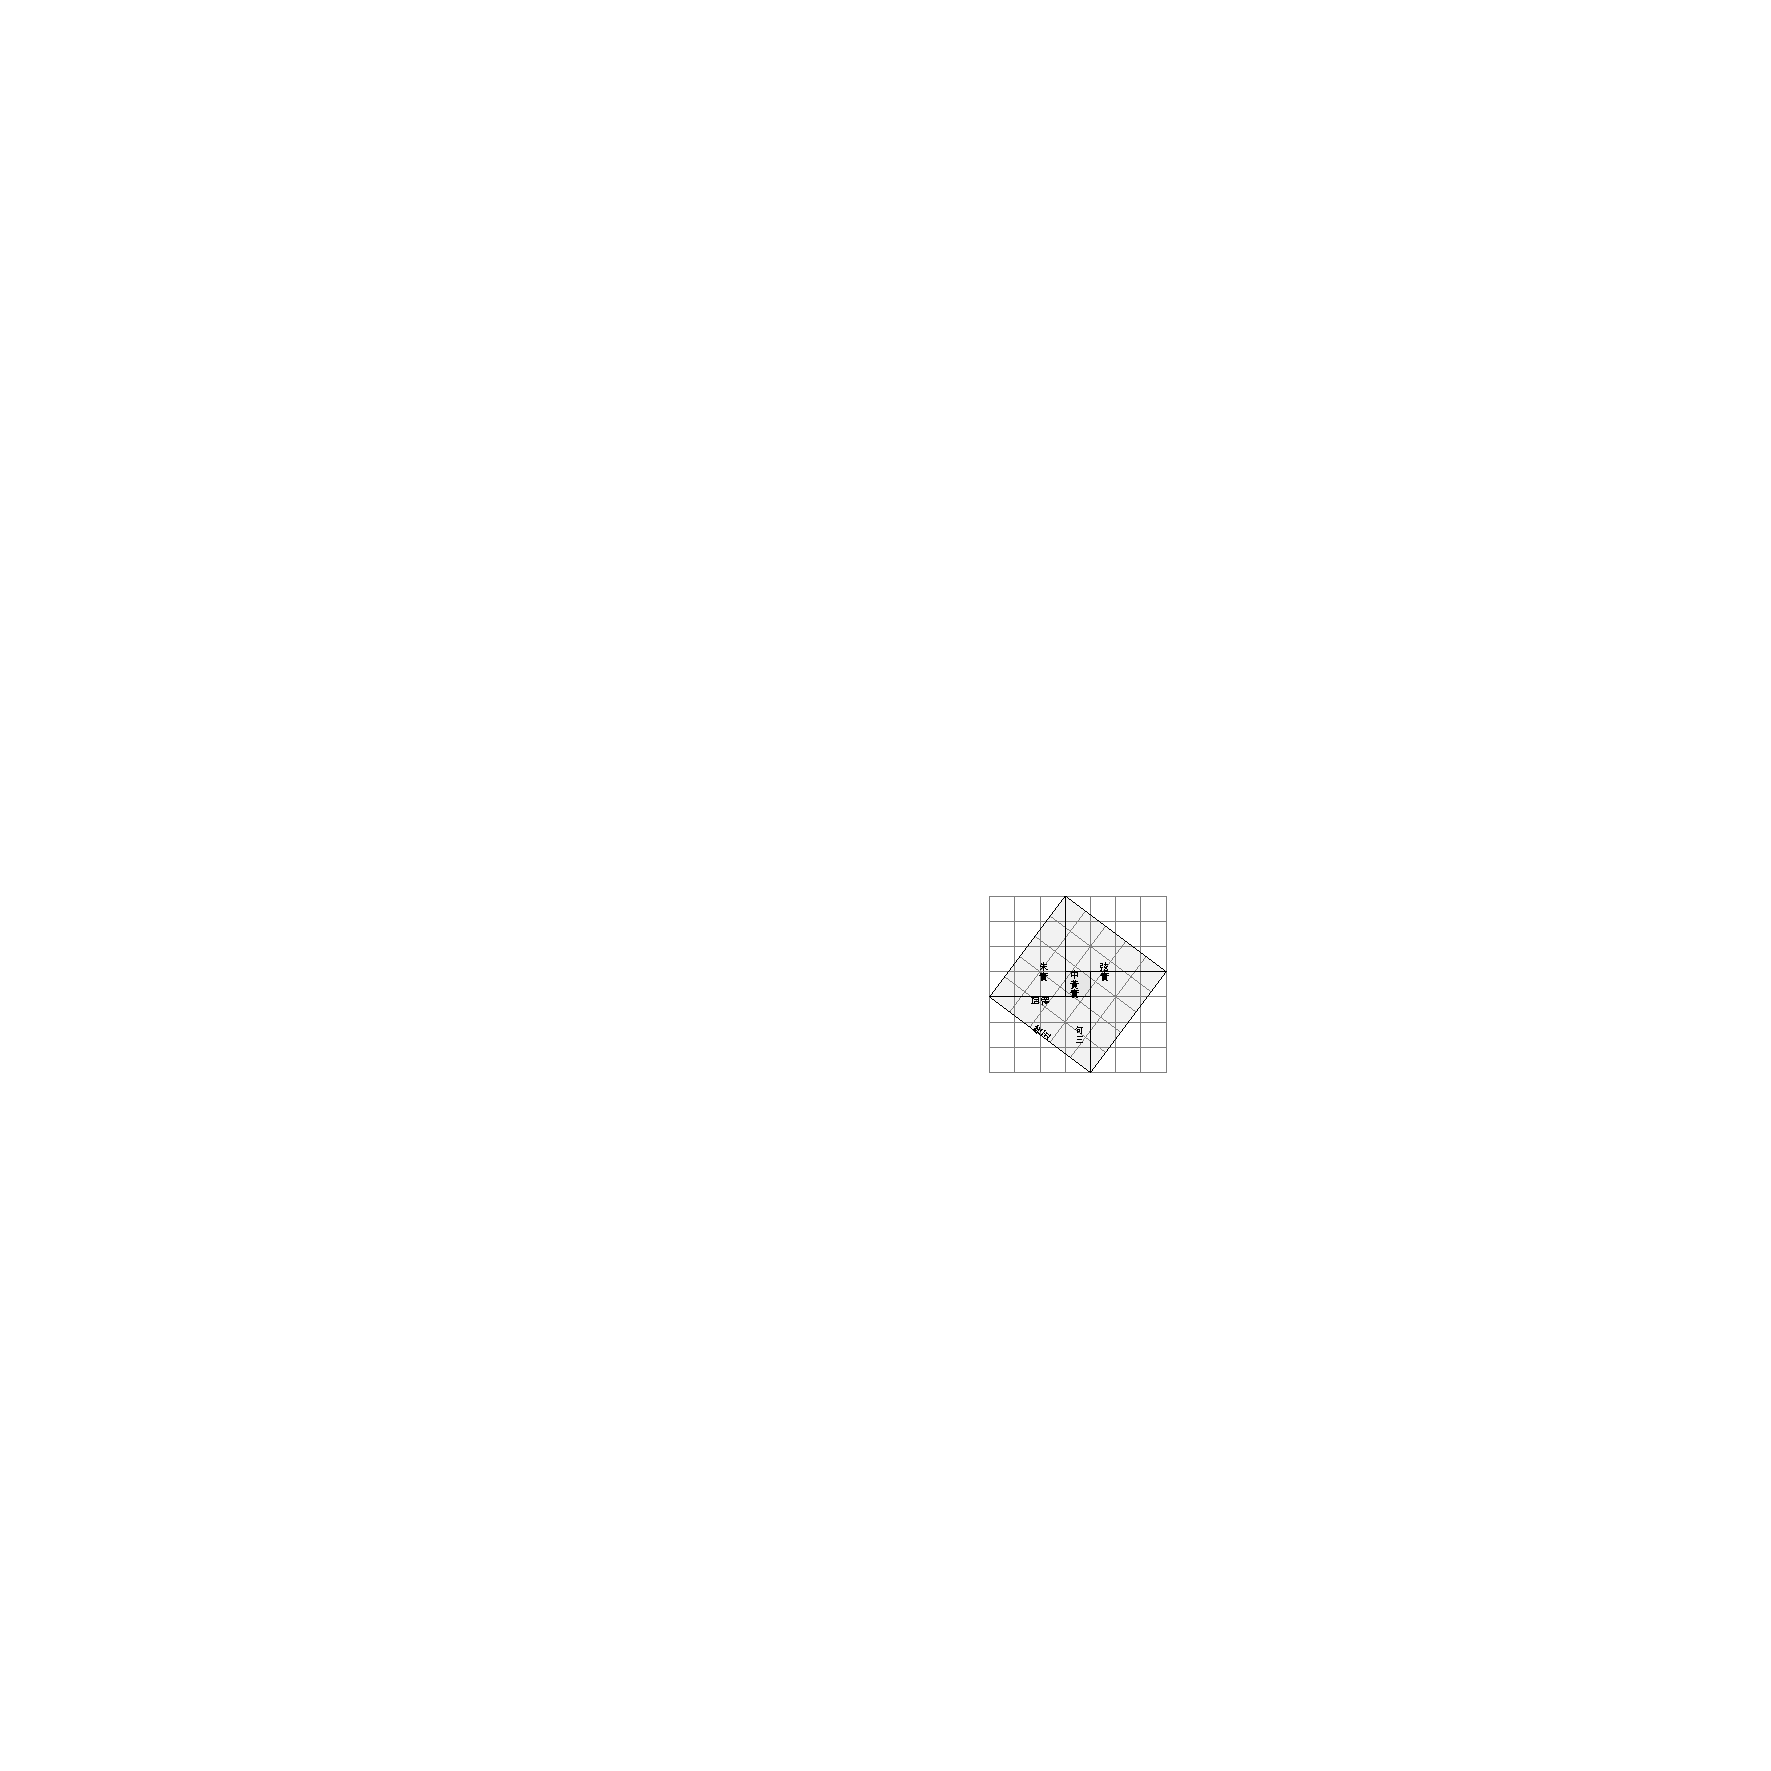
\includegraphics[width=3cm]{xiaotu.pdf}
		
		\begin{figure}[ht]
			\centering
			\includegraphics[scale=0.6]{xiantu.pdf}
			\caption{宋赵爽在《周髀算经》注中作的弦图(仿制),该图给出了勾股定理的一个极具对称美的证明。}
			\label{fig:xiantu}
		\end{figure}
	\end{verbatim}
\end{frame}

\begin{frame}[fragile]{从一个例子说起}{使用图表}
	\begin{verbatim}
		\begin{tabular}{|rrr|}
			\hline
			直角边 $a$ & 直角边 $b$ & 斜边 $c$ \\
			\hline
			3 &4 &5 \\
			5 &12 &13 \\
			\hline
		\end{tabular}
	\end{verbatim}
\end{frame}

\begin{frame}[fragile]{从一个例子说起}{使用图表}
	\begin{verbatim}
		\usepackage{float}% 导言区
		
		\begin{table}[H]
		\begin{tabular}{|rrr|}
		\hline
		直角边 $a$ & 直角边 $b$ & 斜边 $c$\\
		\hline
		3 & 4 & 5 \\
		5 & 12 & 13 \\
		\hline
		\end{tabular}%
		\qquad
		($a^2 + b^2 = c^2$)
		\end{table}
	\end{verbatim}
\end{frame}

\section{自动化工具}

\begin{frame}[fragile]{从一个例子说起}{自动化工具}
	\begin{columns}
	\begin{column}{.5\linewidth}\begin{verbatim}
		% Encoding: UTF8
		
		@ARTICLE{quanjing,
			author = {曲安京},
			title = {商高、赵爽与刘徽关于勾股定理的证明},
			journal = {数学传播},
			year = {1998},
			volume = {20},
			number = {3}
		}
	\end{verbatim}\end{column}

	\begin{column}{.5\linewidth}\begin{verbatim}
		@BOOK{Kline,
			title = {古今数学思想},
			publisher = {上海科学技术出版社},
			year = {2002},
			author = {克莱因}
		}
		@BOOK{Shiye,
			title = {几何的有名定理},
			publisher = {上海科学技术出版社},
			year = {1986},
			author = {矢野健太郎}
		}
	\end{verbatim}\end{column}
	\end{columns}
\end{frame}

\begin{frame}[fragile]{从一个例子说起}{自动化工具}
	\begin{verbatim}
		xelatex gougu.tex
		bibtex gougu.tex
		xelatex gougu.tex
		xelatex gougu.tex
	\end{verbatim}
\end{frame}

\begin{frame}[fragile]{从一个例子说起}{自动化工具}
	\begin{verbatim}
		西方称勾股定理为毕达哥拉斯定理,将勾股定理的发现归功于公元前 6 世纪的毕达哥拉斯学派 \cite{Kline}。
		
		……是我国古代对勾股定理的一种证明 \cite{quanjing}。
		
		\nocite{Shiye}
		\bibliography{math}
		
		图 \ref{fig:xiantu} 是我国古代对勾股定理的一种证明
		\cite{quanjing}。
	\end{verbatim}
\end{frame}

\begin{frame}[fragile]{从一个例子说起}{自动化工具}
	\begin{verbatim}
		\begin{equation}\label{eq:gougu}
			AB^2 = BC^2 + AC^2.
		\end{equation}
		
		% 导言区使用 \usepackage{amsmath}
		满足式 \eqref{eq:gougu} 的整数称为\emph{勾股数}。
	\end{verbatim}
\end{frame}

\begin{frame}[fragile]{从一个例子说起}{自动化工具}
	\begin{verbatim}
		\begin{equation}\label{eq:gougu}
			AB^2 = BC^2 + AC^2.
		\end{equation}
		
		% 导言区使用 \usepackage{amsmath}
		满足式 \eqref{eq:gougu} 的整数称为\emph{勾股数}。
	\end{verbatim}
\end{frame}

\section{设计文章的格式}

\begin{frame}[fragile]{从一个例子说起}{设计文章的格式}
	\begin{verbatim}
		\usepackage{geometry}
		\geometry{a6paper,centering,scale=0.8}
		
		\usepackage[format=hang,font=small,textfont=it]{caption}
		
		\usepackage[nottoc]{tocbibind}
		
		\title{\heiti 杂谈勾股定理}
		\author{\kaishu 张三}
		\date{\today}
	\end{verbatim}
\end{frame}

\begin{frame}[fragile]{从一个例子说起}{设计文章的格式}
	\begin{verbatim}
		\newenvironment{myquote}
		{\begin{quote}\kaishu\zihao{-5}}
		{\end{quote}}
	
		\begin{myquote}
		勾广三,股修四,径隅五。
		\end{myquote}
	
		\newcommand\degree{^\circ}
	\end{verbatim}
\end{frame}

\end{document}